\documentclass[12pt, dvipdfmx]{beamer}

\renewcommand{\kanjifamilydefault}{\gtdefault}
%%%%%%%%%%%  package  %%%%%%%%%%%
\usepackage{bxdpx-beamer}% dvipdfmxなので必要
\usepackage{pxjahyper}% 日本語で'しおり'したい

\usepackage{amssymb,amsmath,ascmac}

\usepackage{multirow}
\usepackage{bm}

\graphicspath{{../../_Figures//}{../../_Figures/Rheology/}}

\usepackage{tikz}
\usepackage{xparse}

\usetikzlibrary{shapes,arrows}
%% define fancy arrow. \tikzfancyarrow[<option>]{<text>}. ex: \tikzfancyarrow[fill=red!5]{hoge}
\tikzset{arrowstyle/.style n args={2}{inner ysep=0.1ex, inner xsep=0.5em, minimum height=2em, draw=#2, fill=black!20, font=\sffamily\bfseries, single arrow, single arrow head extend=0.4em, #1,}}
\NewDocumentCommand{\tikzfancyarrow}{O{fill=black!20} O{none}  m}{
\tikz[baseline=-0.5ex]\node [arrowstyle={#1}{#2}] {#3 \mathstrut};}

%目次スライド
\AtBeginSection[]{
  \frame{\tableofcontents[currentsection]}
}

%アペンディックスのページ番号除去
\newcommand{\backupbegin}{
   \newcounter{framenumberappendix}
   \setcounter{framenumberappendix}{\value{framenumber}}
}
\newcommand{\backupend}{
   \addtocounter{framenumberappendix}{-\value{framenumber}}
   \addtocounter{framenumber}{\value{framenumberappendix}} 
}

%%%%%%%%%%%  theme  %%%%%%%%%%%
\usetheme{Copenhagen}
% \usetheme{Metropolis}
% \usetheme{CambridgeUS}
% \usetheme{Berlin}

%%%%%%%%%%%  inner theme  %%%%%%%%%%%
% \useinnertheme{default}

% %%%%%%%%%%%  outer theme  %%%%%%%%%%%
\useoutertheme{default}
% \useoutertheme{infolines}

%%%%%%%%%%%  color theme  %%%%%%%%%%%
%\usecolortheme{structure}

%%%%%%%%%%%  font theme  %%%%%%%%%%%
\usefonttheme{professionalfonts}
%\usefonttheme{default}

%%%%%%%%%%%  degree of transparency  %%%%%%%%%%%
%\setbeamercovered{transparent=30}

% \setbeamertemplate{items}[default]

%%%%%%%%%%%  numbering  %%%%%%%%%%%
% \setbeamertemplate{numbered}
\setbeamertemplate{navigation symbols}{}
\setbeamertemplate{footline}[frame number]


\title
[レオロジーをはじめる前に]
{レオロジーをはじめる前に}
\author[東亞合成 佐々木]{佐々木 裕\thanks{hiroshi\_sasaki@mail.toagosei.co.jp}}
\institute[東亞合成]{東亞合成株式会社}
\date{}

\begin{document}

%%%%%
% 1 P
%%%%%
\maketitle

%%%%%
% 2 P
%%%%%
%% 目次 (必要なければ省略)
\begin{frame}
\frametitle{Outline}
\tableofcontents
\end{frame}

\begin{frame}
	\frametitle{この章でのお話}
		ここでは、「レオロジーをはじめる前に」として、レオロジーを理解するために必要となる準備を行っていきます。
		具体的には、数学及び物理の基本となるような考え方についての確認から手を付けていきます。
			\begin{itemize}
				\item 数学的な事項の確認
				\begin{itemize}
					\item 数学的に書き表すときに基本となる「関数」について
					\item 事象を単純化して考えるときに重要な「線型性」
				\end{itemize}
				\item 物理的に考えるときに必要になること
				\begin{itemize}
					\item 物理モデルと線形性
					\item 物理モデルを理解するために、「量」、「次元」、「単位」
				\end{itemize}
			\end{itemize} 
\end{frame}

\section{数学的な事項の確認から}
\subsection{関数について}
\begin{frame}
	\frametitle{関数について}
		% \Large
		まず、関数を直感的に理解することから始めましょう。
		\begin{block}{関数の直感的理解}
			\begin{itemize}
				\item 関数とは、
				\begin{itemize}
					% \Large
					\item 2つの変数 $x$ と $y$ があるとしたら、
					\item 入力を $x$ で表したときに、
					\item その出力 $y$ を決定する規則というようなイメージ
				\end{itemize}
				% \Large
				\item 一般に、関数は、
				\begin{itemize}
					\item 英語の function の頭文字を使って $f$ と表記。
					\item そのときに、入力の変数を明示的に $f(x)$ と表す。
				\end{itemize}
			\end{itemize}
		\end{block}
\end{frame}

\begin{frame}
	\frametitle{関数について}
		% \large
		\begin{block}{関数のイメージ}
			\begin{itemize}
				\item ある変数 $x$ に依存して決まる出力 $y$ を\\ 
				\textcolor{red}{決める方法(図の右上)}
				\item 入力 $x$ に対して出力 $y$ を与える\\
				\textcolor{red}{変換装置(図の右下)}
			\end{itemize}
		\end{block}
		\begin{columns}[T, onlytextwidth]
			\column{.48\linewidth}
				\begin{exampleblock}{数式では}
					入力 $x$ と出力 $y$ との関係を\\表現する数式
				\begin{align*}
					y&=f(x) \\
					\text{出力}&=\text{関数} \left(\text{入力} \right)
				\end{align*}
				\end{exampleblock}
			\column{.48\linewidth}
				\vspace{-5mm}
				\begin{center}
					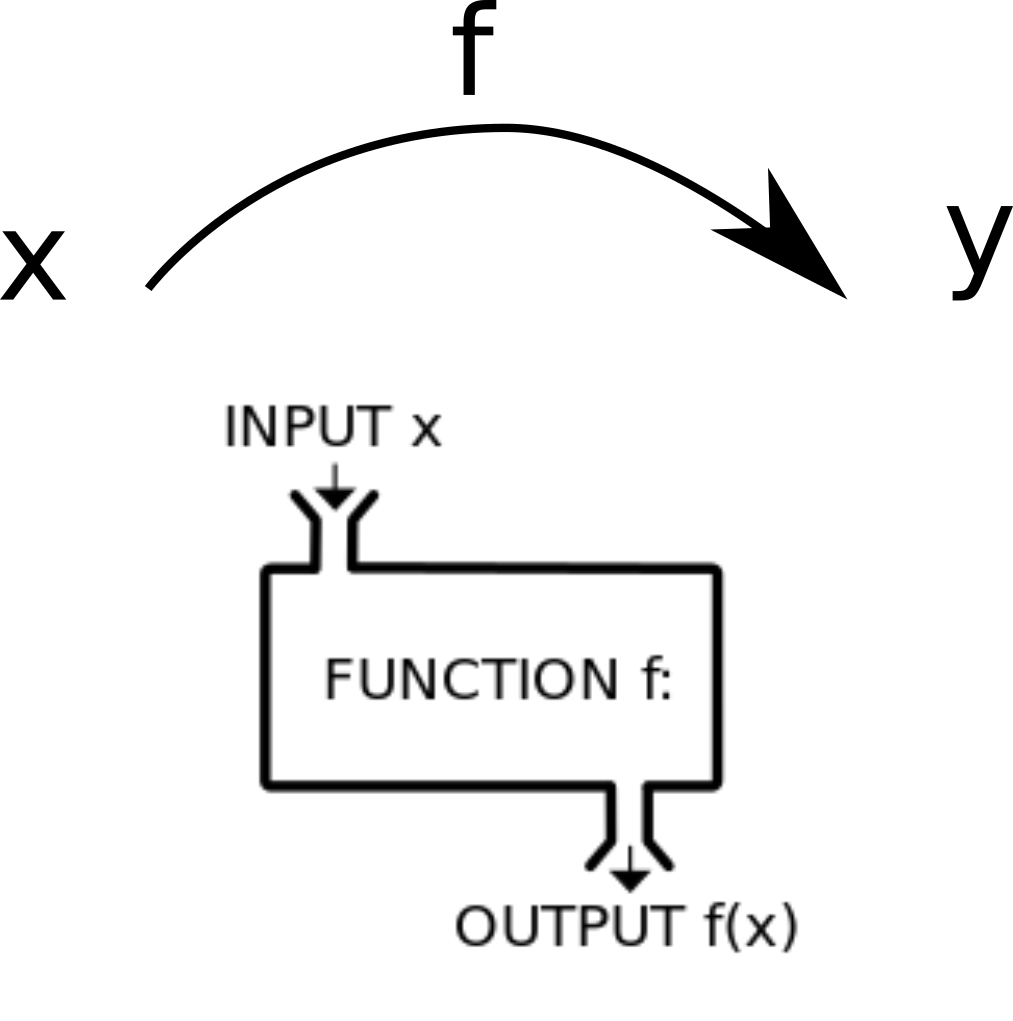
\includegraphics[width=.7\textwidth]{function.png}
				\end{center}
		\end{columns}
\end{frame}

\begin{frame}
	\frametitle{関数と写像}
	関数は、2つの数の集合に値の関連性を与える取る写像の一種と考えることもできます。
	\begin{columns}[T, onlytextwidth]
		\column{.48\linewidth}
			\begin{block}{集合と写像}
				\begin{itemize}
					\item 左の集合から
					\item 右の集合へ
					\item 射影する方法
				\end{itemize}
			\end{block}
		\column{.48\linewidth}
		\begin{center}
			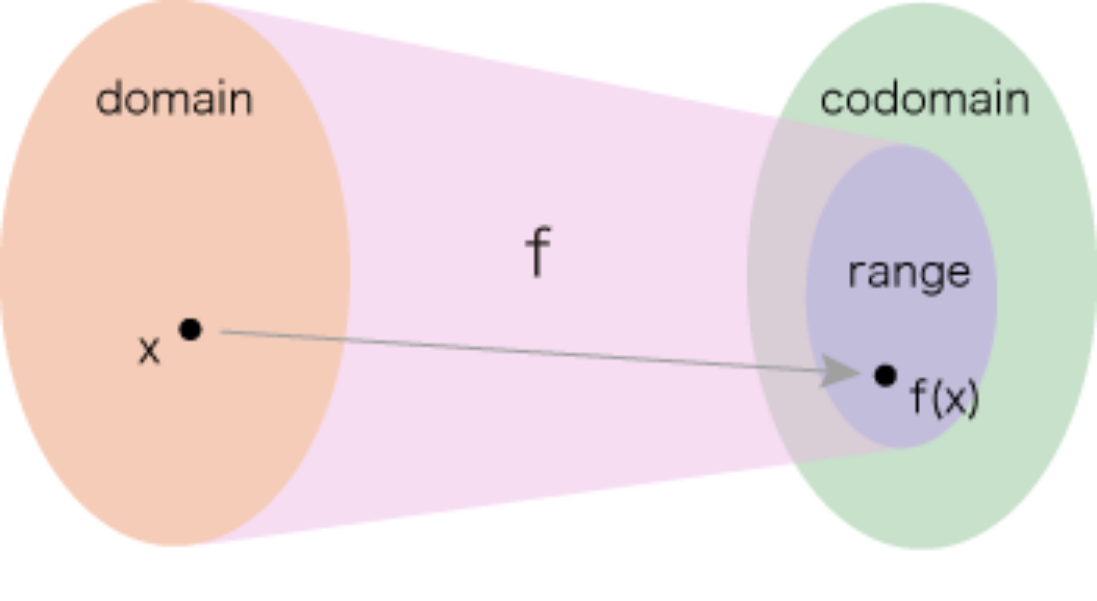
\includegraphics[width=\textwidth]{function_2.png}
			\end{center}
	\end{columns}
\end{frame}

\begin{frame}
	\frametitle{関数とグラフ}
	\begin{block}{グラフとは}
		\begin{itemize}
			\item \alert{入力と出力との関係を平面図}に示したもの
			\item 視覚的に入力と出力との関係を理解しやすくしたもの
			\item 具体的には、
			\begin{itemize}
				\item 入力 $x$ に対応して決まる出力の点を平面上に書き込む
				\item それを連続的に(直線または曲線で)つないだもの
			\end{itemize}
		\end{itemize}
	\end{block}
	\begin{columns}[T, onlytextwidth]
		\column{.48\linewidth}
			\begin{itemize}
				\item 関数を表すグラフ
				\begin{itemize}
					\item 横軸が入力
					\item 縦軸が出力
					\item 赤い曲線が関数
				\end{itemize}
			\end{itemize}
		\column{.48\linewidth}
			\vspace{-5mm}
			\begin{center}
			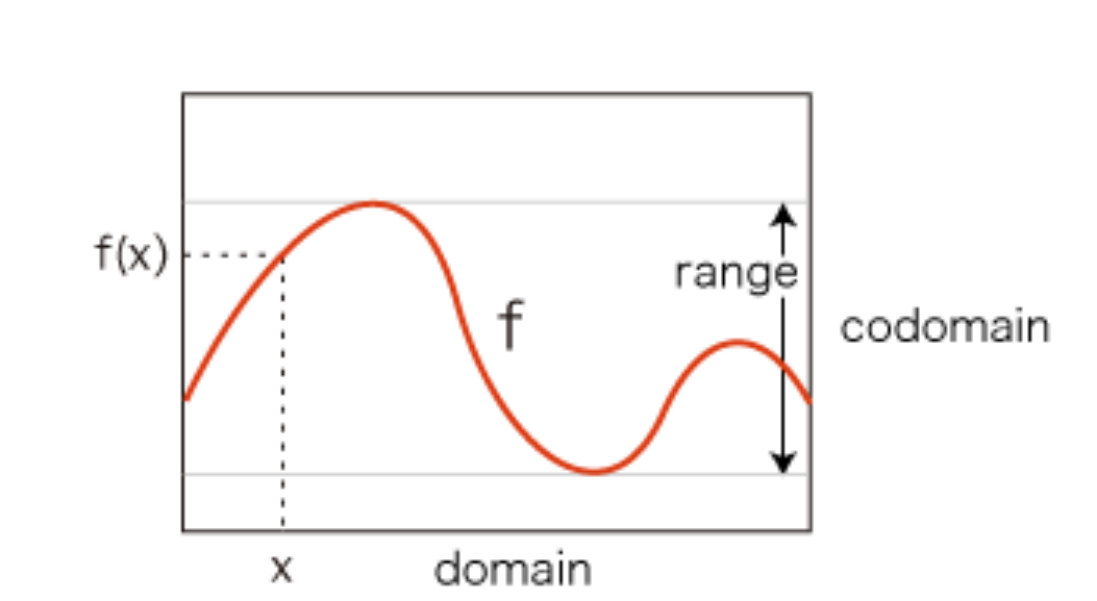
\includegraphics[width=\textwidth]{function_3.png}
			\end{center}
	\end{columns}
\end{frame}
	
\subsection{線型という意味を理解しよう}
\begin{frame}
	\frametitle{線型性とは}
	線型という言葉を直感的にイメージすると、\\\alert{「グラフに表した時に原点を通る直線となる性質」}\\と捉えることができます。
	\begin{block}{数学的な線型性の定義}
		演算(写像)$f$ が、以下に示した2つの性質を満たすとき
		\begin{itemize}
			\item 加法性:任意の $x,y$ に対して、
			\begin{align*}
				f(x+y)=f(x)+f(y)
			\end{align*}
			\item 斉次性:任意の $x,a$ に対して、
			\begin{align*}
				f(ax)=af(x)
			\end{align*}
		\end{itemize}
	\end{block}
\end{frame}

\begin{frame}
	\frametitle{線型性とは}
		\begin{itemize}
			\item 線型性を示す関数はたくさんあります。
			\begin{itemize}
				\item 以下の一次方程式が代表的
					\begin{align*}
						y=ax
					\end{align*}
				\item 比例の関係:入力の大きさが二倍 $\Leftrightarrow$ 出力も二倍
			\end{itemize}
			\item 加法性を利用し、小学校の応用問題としての旅人算も
		\end{itemize}

	\begin{block}{旅人算の例}
		例えば、「A君とB君が 3km 離れた地点から向かい合って同時に出発しました。
		A君は毎分 30m、B君は毎分 70m で歩いたとすると、二人が出会うのは出発してから何分後ですか。」
		というような問題です。
	\end{block}
\end{frame}

\begin{frame}
	\frametitle{線型性の意味}
		% 小学校レベルの簡単な問題を考えてみましょう。
		\begin{itemize}
			\item 「水道の栓を開けて、浴槽に水を溜めています。5 分間流して、100L の水が溜まりました。」
			\begin{itemize}
				\item 「1 分間流したときには、何 L 溜まっていた?」\\
				比例より、 $1 \text{分} \times 100 L /5 \text{分}= 20 L$ ⇔ \textcolor{red}{過去を推定}
				\item「10 分では、何 L 溜まるでしょう?」⇔ \textcolor{red}{未来を予測}
			\end{itemize}
			\item 「二つの蛇口から水を溜め、A 蛇口からは 1 分間で 20 L、B 蛇口は 5 分間で 150 L の水を貯められる。」
			\begin{itemize}
				\item 「両方の蛇口から同時だと、10 分間では何 L?」
				\item \textcolor{red}{加法性と斉次性を利用}すれば簡単に解ける
			\end{itemize}
		\end{itemize}
		\begin{alertblock}{線型性の意味}
			線型性が成立する(と仮定する)ことで、
			\begin{itemize}
				\item 事象を重ね合わせながら
				\item 過去や未来の値を決定
			\end{itemize}
		\end{alertblock}
\end{frame}

\section{物理的に考えましょう}
\subsection{物理モデルと線型性}
\begin{frame}
	\frametitle{物理モデルについて}
	% \Large
	% 続いて、物理モデルとの関係で考えてみましょう。
	\begin{exampleblock}{物理モデルという考え方}
		\begin{itemize}
			\item モデルという言葉の意味は?\\
			\alert{「事象や理論の成り立ちを説明するための\\理解しやすい概念(考え方)」}
			\begin{itemize}
				\item 「地動説」を説明するために、「太陽系モデル」が提案
				\item 経済活動で利益の最大化に種々の「ビジネスモデル」
			\end{itemize}
			\item \alert{「モデルとは、対象とする事象を簡略化して、\\その本質を表したもの」}という表現も。
			\begin{itemize}
				\item 対象を物理現象にとったとき、「物理モデル」
				\item 定量的な解析のために数学を応用した「数理モデル」\\
				$\Rightarrow$ モデル化で使った概念を数式表現へ落とし込む
			\end{itemize}
		\end{itemize}
	\end{exampleblock}
	% 我々の議論においては、レオロジーに関連する理論を説明するために使える考え方やイメージ図として物理モデルを利用して理解を深めていくわけです。
\end{frame}

\begin{frame}
	\frametitle{物理現象と線型応答}
	\begin{itemize}
		\item 我々の身の回りに起こっている実際の事柄
		\begin{itemize}
			\item 非常に複雑な場合がほとんど
			\item 評価したい出力(応答)も分かりづらい
			\item 入力も不明確だったりする
		\end{itemize}
		\item 入力が小さい場合
		\begin{itemize}
			\item 応答が線型で取り扱える場合が多い
			\begin{itemize}
				\item 加法性や斉次性が使える
				\item 入力が多種類となってもそれらが分割可能\footnote{
					ここでは、詳しくは説明しませんが、分割できるということは独立に起きている事柄ということになります。
				}
			\end{itemize}
			\item 取り扱いたい事象の細かい部分を無視
		\end{itemize}
		\alert{\item 単純化(近似)して理解}
	\end{itemize}
\end{frame}

\begin{frame}
	\frametitle{物理モデルと線型性}
		\begin{alertblock}{簡単なまとめ}
			\begin{itemize}
				\item 実際の身の回りの現象
				\begin{itemize}
					\item \textcolor{blue}{非常に複雑}な場合がほとんど。
					\item 評価したい応答も分かり難い。
					\item 入力すら不明確なときも。
				\end{itemize}
				\item 線型現象であれば、取り扱いが容易。
				\begin{itemize}
					\item \textcolor{red}{微小な刺激に対しては、線形応答が期待}できる。
					\item 線形応答の重ね合わせで、\textcolor{red}{事象を近似}する価値は高い。
				\end{itemize}
				\item 線型性が成り立っているのであれば、
				\begin{itemize}
					\item 比例定数を調べることで
					\item 物質の性質を\textcolor{red}{容易に比較}できる
				\end{itemize}
			\end{itemize}	
		\end{alertblock}
		\normalsize
		ここでは、線型性を仮定できるような単純な物理モデルを利用して理解を深めていきます。
\end{frame}

\subsection{物理モデルを理解するために、「量」、「次元」、「単位」}
\begin{frame}
	\frametitle{物理モデルを理解するために}
	まず、天下りに、「量とは」を考えてみます。
	\begin{block}{量とは}
		\begin{itemize}
			\item 我々が物事の評価を行うときに、
			\begin{itemize}
				\item 「定性的に考えて区別」するために、
				\item 「定量的に決定できる」もの
			\end{itemize}
			\item そして、物理的に考えるときには、
			\begin{itemize}
				\item 「次元が決まって」、
				\item 「定められた単位の倍数」として表す
			\end{itemize}
			\item 工学的には、「測定方法によって定義」される
		\end{itemize}
	\end{block}
	ですから、量というものを、次元と単位、そして、測定方法を定義しながら、議論することが必要となります。
\end{frame}

\begin{frame}
	\frametitle{「量」、「次元」、「単位」の定義}
	\footnotesize
	\begin{exampleblock}{「計測用語」についてまとめた JIS Z 8103 では}
		\begin{description}
			\item[量] 現象、物体又は物質の持つ属性で、定性的に区別でき、かつ、定量的に決定できるもの。
			\item[物理量] 物理学における一定の理論体系の下で次元が確定し、定められた単位の倍数として表すことができる量。
			\item[工学量] 複数の物理的性質に関係する量で、測定方法によって定義される工業的に有用な量。硬さ、表面粗さ等。
			\item[量の次元] ある量体系に含まれるある一つの量を、その体系の基本量を表す因数のべき乗の積として示す表現。
			\item[量体系] 一般的な意味で、定まった関係が存在する量の集合。
			\item[単位] 取決めによって定義され、採用された特定の量であって、同種の他の量の大きさを表すために比較されるもの。
		\end{description}
	\end{exampleblock}
\end{frame}

\begin{frame}
	\frametitle{量の性質}
	\begin{exampleblock}{量の演算}
		\begin{itemize}
			\item \textcolor{red}{同じ種類の量同士は和と差}の演算が定義可能
			\begin{itemize}
				\item 結果は同じ種類の量
				\item 足したり引いたりすることでその大きさが変化
				\item \textcolor{red}{異なる種類の量の和や差には意味がない}
			\end{itemize}
			\item 同じ、あるいは、異なる種類の量同士でも、\\ \textcolor{red}{積や商が定義}できることがあり、
			\begin{itemize}
				\item 長さ同士の積は面積
				\item 長さの時間による商は速さ
			\end{itemize}
		\end{itemize}
	\end{exampleblock}
\end{frame}

\begin{frame}
	\frametitle{量の次元}
	\begin{itemize}
		\item 先程示した定義で「量の次元」は、
		\begin{itemize}
			\item 「ある量体系に含まれるある一つの量を、その体系の基本量を表す因数のべき乗の積として示す表現。」
			\item \textcolor{blue}{よくわからない。}
		\end{itemize}
		\item 言葉を足して言い換えてみると、
		\begin{itemize}
			\item 「何らかの関係が成り立つ量の集合において、一つの量を、その関係の基本となる量の種類とそのべき乗だけで表す考え方」
			\item \textcolor{blue}{これでもわかりにくい}
		\end{itemize}
	\end{itemize}
	\begin{exampleblock}{もっと直感的な「次元」のイメージ}
		「次元」とは、複合的なイメージとしての「ある量」を、「基本量の積と商で表す」考え方のこと。
	\end{exampleblock}
\end{frame}

\begin{frame}
	\frametitle{国際量体系での定義}

	国際量体系(ISQ: International System of Quantities)の体系に従って、表のように7つの基本量が定められています。
	\begin{center}
		\begin{tabular}{|c|c||c|c|} \hline
			基本量 		& 次元の記号 & SI単位 		& 単位の記号\\ \hline \hline
			長さ		& L			& メートル 		& m \\ \hline
			質量		& M			& キログラム 	& kg \\ \hline
			時間		& T			& 秒 			& s \\ \hline
			電流		& I			& アンペア 		& A \\ \hline
			熱力学温度	& $\Theta$	& ケルビン 		& K \\ \hline
			物質量		& N			& モル 			& mol \\ \hline
			光度		& J			& カンデラ 		& cd \\ \hline
		\end{tabular}
	\end{center}
\end{frame}

\begin{frame}
	\frametitle{次元の関係式}
	\footnotesize
	\begin{itemize}
		\item 量 $\mathrm{Q}$ の次元は、角括弧で括って $[\mathrm{Q}]$ で表記する
		\item このとき、長さという基本量に関わる量体系は、
			\begin{align*}
				\begin{cases}
					[\text{面積}] = [\text{長さ}]^2 = [\mathrm{L}^2] \\[8pt]
					[\text{体積}] = [\text{長さ}]^3 = [\mathrm{L}^3]
				\end{cases}
			\end{align*}
		\item 力学に関係する物理量は異種の基本量の組み合わせで、
			\begin{align*}
				\begin{cases}
					[\text{速さ}] = [\text{長さ}][\text{時間}]^{-1} = [\mathrm{LT}^{-1}] \\[8pt]
					[\text{加速度}] = [\text{長さ}][\text{時間}]^{-2} = [\mathrm{LT}^{-2}] \\[8pt]
					[\text{力}] = [\text{質量}][\text{長さ}][\text{時間}]^{-2} = [\mathrm{MLT}^{-2}]
					%  \\[8pt]
					% [\text{仕事}] = [\text{質量}][\text{長さ}]^2[\text{時間}]^{-2} = [\mathrm{ML}^2\mathrm{T}^{-2}]
				\end{cases}
				\label{eq:idou}
			\end{align*}
		\item 次元の関係式とは「定数係数を無視した等式として表すことで物理現象の成り立ちを表している」
	\end{itemize}
\end{frame}

\begin{frame}
	\frametitle{単位について}
	\begin{itemize}
		\item 単位とは、
		\begin{itemize}
			\item 「取決めによって定義された同種の物理量の大きさを表す」
		\end{itemize}
		\item 標準となる単位系は、
		\begin{itemize}
			\item 国際単位系(SI)
			\footnote{仏: Syst\`eme International d'Unit\'es、英: International System of Units、フランス語の略称なので SI となる。}
			\item 次元の基本量に対応した7つの基本単位
		\end{itemize}
		\item 任意の物理量の値 $Q$ は、
		\begin{itemize}
			\item その大きさを表す数値 $n$ と単位 $U$ との積
			\item 単位のとり方に依存して、数値は変更を受ける
			\begin{itemize}
				\item 例えば、時間の単位として「秒」で表して定数係数が\\大きすぎる場合は、「時」、「年」等も用いる
				\item 臨機応変に対応しましょう。
			\end{itemize}
		\end{itemize}
	\end{itemize}
\end{frame}

\begin{frame}
	\frametitle{組立単位}
	\begin{itemize}
		\item 組立単位
		\begin{itemize}
			\item 基本単位の組み合わせで、
			\item 固有の名称と記号で表される
			\item SI 組立単位としては、22 個
		\end{itemize}
	\end{itemize}
	レオロジーに関連する主要なものは、
	\vspace{-3mm}
	\small
	\begin{center}
		\begin{tabular}{|c|c||c|c|} \hline
			組立量 		& 名称					& 記号		& SI 基本単位による表現 	\\ \hline \hline
			周波数		& ヘルツ (hertz)		& Hz		&  s$^{-1}$ 					\\ \hline
			力			& ニュートン (newton)	& N 		& m$\cdot$kg$\cdot$s$^{-2}$ 	\\ \hline
			応力		& パスカル (pascal)		& Pa 		& (N/m$^2$) = m$^{-1}\cdot$kg$\cdot$s$^{-2}$ \\ \hline
			エネルギー	& ジュール (joule)		& J 		& (N$\cdot$m) = m$^{2}\cdot$kg$\cdot$s$^{-2}$ \\ \hline
			粘度		& パスカル秒			& Pa$\cdot$s & m$^{-1}\cdot$kg$\cdot$s$^{-1}$ \\ \hline
		\end{tabular}
	\end{center}
\end{frame}

\begin{frame}
	\frametitle{まとめ}
	ここでは、レオロジーを理解するために必要となる準備を行いました。
	\begin{boxnote}
		\begin{itemize}
			\item 数学的な事項の確認
			\begin{itemize}
				\item 数学的に書き表すときに基本となる「関数」
				\item 事象の単純化に重要な「線型性」
			\end{itemize}
			\item 物理的に考えるときに必要になること
			\begin{itemize}
				\item 物理モデルと線形性
				\item 「量」、「次元」、「単位」
			\end{itemize}
		\end{itemize} 
	\end{boxnote}
\end{frame}

% \appendix
% \backupbegin

% \section{演習問題 1}
% \subsection{「関数について」}
% \begin{frame}
% 	\frametitle{「関数について」}
% 	% \scriptsize
% 	% 以下の穴を埋めてください。
% 		\begin{itemize}
% 			\item \textcolor<2>{black}{関数}の役割を考えてみると、\fbox{\textcolor<1>{white}{入力}}を変換装置に入れた結果として\fbox{\textcolor<1>{white}{出力}}が現れるわけですから、入力と出力との間の\fbox{\textcolor<1>{white}{関係}}を表していると考えることもできます。
% 			\item また、関数というのは、\fbox{\textcolor<1>{white}{数の集合}}に値を取る\fbox{\textcolor<1>{white}{写像}}の一種と考えることもできます。
% 			\item グラフとは、\fbox{\textcolor<1>{white}{入力}}と\fbox{\textcolor<1>{white}{出力}}との関係を\fbox{\textcolor<1>{white}{平面図}}に示したものであり、視覚的にその関係を理解しやすくしたものと考えることができます。
% 			\item このグラフに表した関数の\fbox{\textcolor<1>{white}{形}}を見ることで、入力と出力との\fbox{\textcolor<1>{white}{関係}}を直感的に理解することができます。
% 		\end{itemize}
% \end{frame}

% \subsection{「線型という意味を理解」}
% \begin{frame}
% 	\frametitle{「線型という意味と物理モデル」}
% 	% \scriptsize
% 	% 以下の穴を埋めてください。
% 	\begin{itemize}
% 		\item \textcolor<2>{black}{線型}という言葉は直感的には、\fbox{\textcolor<1>{white}{グラフ}}に表した時に\fbox{\textcolor<1>{white}{原点を通る直線}}となるような性質と捉えられます。
% 		\item これは、入力の大きさが二倍になれば、\fbox{\textcolor<1>{white}{出力も二倍}}になるという比例の関係を表しています。
% 		\item 物理モデルとは、「\fbox{\textcolor<1>{white}{事象や理論の成り立ち}}を説明するための簡単で理解しやすい\fbox{\textcolor<1>{white}{概念や模型}}」です。
% 		\item 我々の身の回りに起こっている実際の事柄は、\fbox{\textcolor<1>{white}{非常に複雑}}な場合がほとんどです。
% 		\item 都合のいいことに、\fbox{\textcolor<1>{white}{入力が小さい}}場合には応答が\fbox{\textcolor<1>{white}{線型}}で取り扱える場合が多いことが知られている。
% 	\end{itemize}
% \end{frame}

% \section{演習問題 2}
% \subsection{「量について」}
% \begin{frame}
% 	\frametitle{「量について」}
% 	% \scriptsize
% 	% 以下の穴を埋めてください。
% 	\begin{itemize}
% 		\item \textcolor<2>{black}{量}とは、現象、物体又は物質の持つ属性で、\fbox{\textcolor<1>{white}{定性的に区別}}でき、かつ、\fbox{\textcolor<1>{white}{定量的に決定}}できるもの。
% 		\item 同じ種類の量同士は\fbox{\textcolor<1>{white}{和と差}}の演算が定義可能
% 		\begin{itemize}
% 			\item 結果は同じ種類の\fbox{\textcolor<1>{white}{量}}
% 			\item \fbox{\textcolor<1>{white}{異なる種類}}の量の和や差には\fbox{\textcolor<1>{white}{意味がない}}
% 		\end{itemize}
% 		\item 同じ、あるいは、異なる種類の量同士でも\fbox{\textcolor<1>{white}{積や商}}が定義できることがあり、
% 		\begin{itemize}
% 			\item 長さ同士の積は\fbox{\textcolor<1>{white}{面積}}
% 			\item 長さの時間による商は\fbox{\textcolor<1>{white}{速さ}}
% 		\end{itemize}
% 	\end{itemize}
% \end{frame}

% \subsection{「次元について」}
% \begin{frame}
% 	\frametitle{「次元について」}
% 	% \scriptsize
% 	% 以下の穴を埋めてください。
% 	\begin{itemize}
% 		\item \textcolor<2>{black}{次元}とは、注目する「ある量」を、「\fbox{\textcolor<1>{white}{基本量}}の\fbox{\textcolor<1>{white}{積と商}}で表す」考え方ともいえます。
% 		\item 国際量体系では、7つの基本量が定められています。レオロジーでよく使う四つの基本量を埋めてください。
% 			% \begin{table}[h]
% 				\begin{center}
% 					\begin{tabular}{|c|c||c|c|} \hline
% 						基本量 		& 次元の記号 & SI単位 		& 単位の記号\\ \hline \hline
% 						\fbox{\textcolor<1>{white}{長さ}}		& L			& メートル 		& m \\ \hline
% 						\fbox{\textcolor<1>{white}{質量}}		& M			& キログラム 	& kg \\ \hline
% 						\fbox{\textcolor<1>{white}{時間}}		& T			& 秒 			& s \\ \hline
% 						電流		& I			& アンペア 		& A \\ \hline
% 						\fbox{\textcolor<1>{white}{熱力学温度}}	& $\Theta$	& ケルビン 		& K \\ \hline
% 						物質量		& N			& モル 			& mol \\ \hline
% 						光度		& J			& カンデラ 		& cd \\ \hline
% 					\end{tabular}
% 				\end{center}
% 			% \end{table}
% 	\end{itemize}
% \end{frame}

% \subsection{「単位について」}
% \begin{frame}
% 	\frametitle{「単位について」}
% 	% \scriptsize
% 	% 以下の穴を埋めてください。
% 	\begin{itemize}
% 		\item \textcolor<2>{black}{単位}を簡単に言えば、「取決めによって定義された\fbox{\textcolor<1>{white}{同種の物理量の大きさ}}を表すため」に使うものです。
% 		\item 現在、最も広く使われている(取決めによって定義された)単位系は、\fbox{\textcolor<1>{white}{国際単位系(SI)}}です。
% 		\item 任意の\fbox{\textcolor<1>{white}{物理量の値}} $Q$ は、その大きさを表す\fbox{\textcolor<1>{white}{数値}} $n$ と単位 $U$ との積として表されることになります。
% 		\item 基本単位の組み合わせとして、固有の名称と記号で表される\fbox{\textcolor<1>{white}{組立単位}}というものもあります。
% 	\end{itemize}
% \end{frame}

% \begin{frame}
% 	\frametitle{「単位について」}
% 			\footnotesize
% 			\begin{center}
% 				% \caption{}
% 				% \label{tab:kumitate2}
% 				\begin{tabular}{|c|c||c|c|} \hline
% 					\textcolor<2>{black}{組立量} 		& 名称					& 記号		& SI 基本単位による表現 	\\ \hline \hline
% 					\fbox{\textcolor<1>{white}{周波数}}		& ヘルツ (hertz)		& Hz		&  s$^{-1}$ 					\\ \hline
% 					\fbox{\textcolor<1>{white}{力}}			& ニュートン (newton)	& N 		& m$\cdot$kg$\cdot$s$^{-2}$ 	\\ \hline
% 					\fbox{\textcolor<1>{white}{応力}}		& パスカル (pascal)		& Pa 		& (N/m$^2$) = m$^{-1}\cdot$kg$\cdot$s$^{-2}$ \\ \hline
% 					\fbox{\textcolor<1>{white}{エネルギー}}	& ジュール (joule)		& J 		& (N$\cdot$m) = m$^{2}\cdot$kg$\cdot$s$^{-2}$ \\ \hline
% 					\fbox{\textcolor<1>{white}{粘度}}		& パスカル秒			& Pa$\cdot$s & m$^{-1}\cdot$kg$\cdot$s$^{-1}$ \\ \hline
% 				\end{tabular}
% 			\end{center}
% 		% \end{table}
% 	% \end{itemize}
% \end{frame}


% \backupend
\end{document}